\section{High-level Computer Architecture Overview}

\label{sec:high}
\subsection{System Review}
To understand distributed systems, we must first review 
the architecture of a single computer.

\begin{Def}[Turing Machine]
    
    Conceptualized by Alan Turing in 1936, a Turing machine is a mathematical model of computation that defines an abstract machine 
    that manipulates symbols on a strip of tape according to a table of rules. Despite its simplicity, the machine can simulate the 
    logic of any computer algorithm.
\end{Def}

\begin{Def}[Vaun Neumann Architecture]
    
    The Von Neumann architecture, also known as the Princeton architecture, is a 
    design architecture for an electronic digital computer with these components:
    \begin{itemize}
        \item \textbf{A processing unit} that contains an arithmetic logic unit and a control unit.
        \item \textbf{A memory unit} that stores data and instructions.
        \item \textbf{Input and output mechanisms}.
    \end{itemize}
\end{Def}

\noindent
Fast forward, modern computers have the following components:
\begin{Def}[Modern Computer Components]

    \begin{itemize}
        \item \textbf{CPU:} Central Processing Unit. The brain of the computer that performs instructions.
        \item \textbf{Memory:} Stores data and instructions.
        \item \textbf{Storage:} Hard drives, SSDs, etc.
        \item \textbf{Network Interface:} Connects the computer to the network.
        \item \textbf{Input/Output Devices (I/O):} Keyboard, mouse, monitor, etc.
        \item \textbf{Motherboard:} The central printed circuit board that interconnects all of the computer's components, including the CPU, storage devices, and I/O devices.
    \end{itemize}
\end{Def}

\newpage 

\noindent 
Before diving deeper into the inner workings of a single computer, let's define a distrusted system:

\begin{Def}[Distributed System]
    
    A distributed system is a system whose components are located on different networked computers, which communicate and coordinate their actions by passing messages to one another. 
    The components interact with one another in order to achieve a common goal.
\end{Def}

\noindent
In the words of Andrew S. Tanenbaum,

\begin{gbox}

\begin{center}
    \textit{``A set of nodes, connected by a
    network, which appear to its users as
    \\a single coherent system.''}\\
\end{center}

\vspace{.5em}
\end{gbox}
\noindent
or in the words of Leslie Lamport,

\begin{gbox}
\begin{center}
    \textit{A distributed system is one in which
    the failure of a computer you didn't
    even know existed can render your
    own computer unusable.}
\end{center}

\vspace{.5em}
\end{gbox}

\begin{Tip}
    \textbf{Andrew S. Tanenbaum} is a computer scientist and professor emeritus at the Vrije Universiteit Amsterdam in the Netherlands who is best known for his books on computer science.
    \textbf{Leslie Lamport} is an American computer scientist known for his work in distributed systems and as the initial developer of the document preparation system \LaTeX.
\end{Tip}

\subsection{CPU and Memory Orchestration Review}
Now at a high-lever, we discuss how the a system interacts with all its components to perform tasks.

\begin{Def}[CPU (Central Processing Unit)]
    
    The CPU is made of the following components:
    \begin{itemize}
        \item \textbf{ALU (Arithmetic Logic Unit):} Performs arithmetic and logical operations.
        \item \textbf{Control Unit:} Manages the execution of instructions.
        \item \textbf{Registers:} Small, fast storage locations in the CPU that temporarily hold data and instructions.
    \end{itemize}
\end{Def}

\newpage

\begin{Def}[Memory Segments]

    A program's memory is typically divided into several segments:
\begin{itemize}
    \item \textbf{Text Segment:} Contains the executable code.
    \item \textbf{Data Segment:} Stores global and static variables.
    \item \textbf{System Stack:} A memory region that manages temporary data related to function calls in a first-in-last-out manner.
    \item \textbf{System Heap:} A memory region that dynamically allocates references to data from the stack memory. 
\end{itemize}
\end{Def}

\begin{Def}[Instruction Execution Cycle]

    The instruction execution cycle, also known as the \emph{fetch-decode-execute} cycle, is the process by which the CPU processes instructions. In each cycle:
\begin{enumerate}
    \item \textbf{Fetch:} The CPU retrieves an instruction from memory using the \emph{instruction pointer} (or program counter).
    \item \textbf{Decode:} The instruction is interpreted to determine what action is required.
    \item \textbf{Execute:} The CPU performs the instruction's operation, which may involve arithmetic calculations, memory accesses, or I/O operations.
\end{enumerate}
\end{Def}

\noindent
The CPU performs instructions via the following steps:
\begin{Def}[CPU Registers]

    Registers are small, high-speed storage locations within the CPU that temporarily hold data, instructions, and control information. Key registers include:
\begin{itemize}
    \item \textbf{Instruction Pointer (Program Counter):} Holds \textbf{addresses}, which are the locations of the next instruction to fetch.
    \item \textbf{Stack Pointer:} Points to the top of the current stack in memory.
    \item \textbf{General-Purpose Registers:} Used for arithmetic operations and temporary data storage.
\end{itemize}
\end{Def}


\newpage 
\begin{Def}[RAM and Volatile Memory]

    RAM (Random Access Memory) is a type of volatile memory used to store data and instructions that are actively used by the CPU. Since it is volatile, its contents are lost when the computer is powered off.
\end{Def}

\begin{Def}[Physical Storage and I/O Devices]

    Physical storage refers to non-volatile memory devices such as hard drives and SSDs, which retain data without power. Many of these devices are accessed via input/output (I/O) operations and are thus considered part of the system's I/O mechanism.
\end{Def}

\begin{Def}[Virtual Memory and Address Translation]

    Virtual memory is a memory management technique that provides an abstraction of a large, contiguous memory space. It works by mapping virtual addresses used by programs to physical addresses in RAM via structures such as page tables, which are managed by the Memory Management Unit (MMU).
\end{Def}

    
\begin{Def}[CPU Cores]

    A CPU core is a physical processing unit within a central processing unit (CPU) responsible for executing instructions and performing computations. Modern CPUs often contain multiple cores, enabling them to handle multiple tasks at the same time. 
\end{Def}

\begin{Def}[Task, Job, and Process]

    \begin{itemize}
        \item A \textbf{Task} is a single unit of work in various states (waiting, running, completed).
        \item A \textbf{Job} is a high-level operation comprising multiple tasks.
        \item A \textbf{Process} is an executing instance of a program that manages system resources instructing the CPU to execute tasks.
    \end{itemize}
\end{Def}

\newpage
\begin{Def}[Threads: Concurrency \& Parallelism]

    A \textbf{thread} is a unit of logic (a segment of code) to be executed by a CPU core. \textbf{A core can only run one thread at a time}.
    The core itself is called the \textbf{hardware-thread}, while our units of logic are called \textbf{software-threads} or \textbf{OS-threads}.

    The OS system scheduler manages the hardware-threads, and assigns software-threads to them. Switching between software-threads on a hardware-thread is called \textbf{context switching}.
    Context switching is expensive, as it requires saving the current state of the software-thread and loading the state of the new software-thread. Though it provides the illusion of tasks running simultaneously, 
    called \textbf{concurrency}.
    
    With multiple cores come \textbf{multi-threading}, where multiple threads run on other cores simultaneously.
    This true simultaneity is called \textbf{parallelism}.
\end{Def}
\begin{figure}[h]
    \centering
    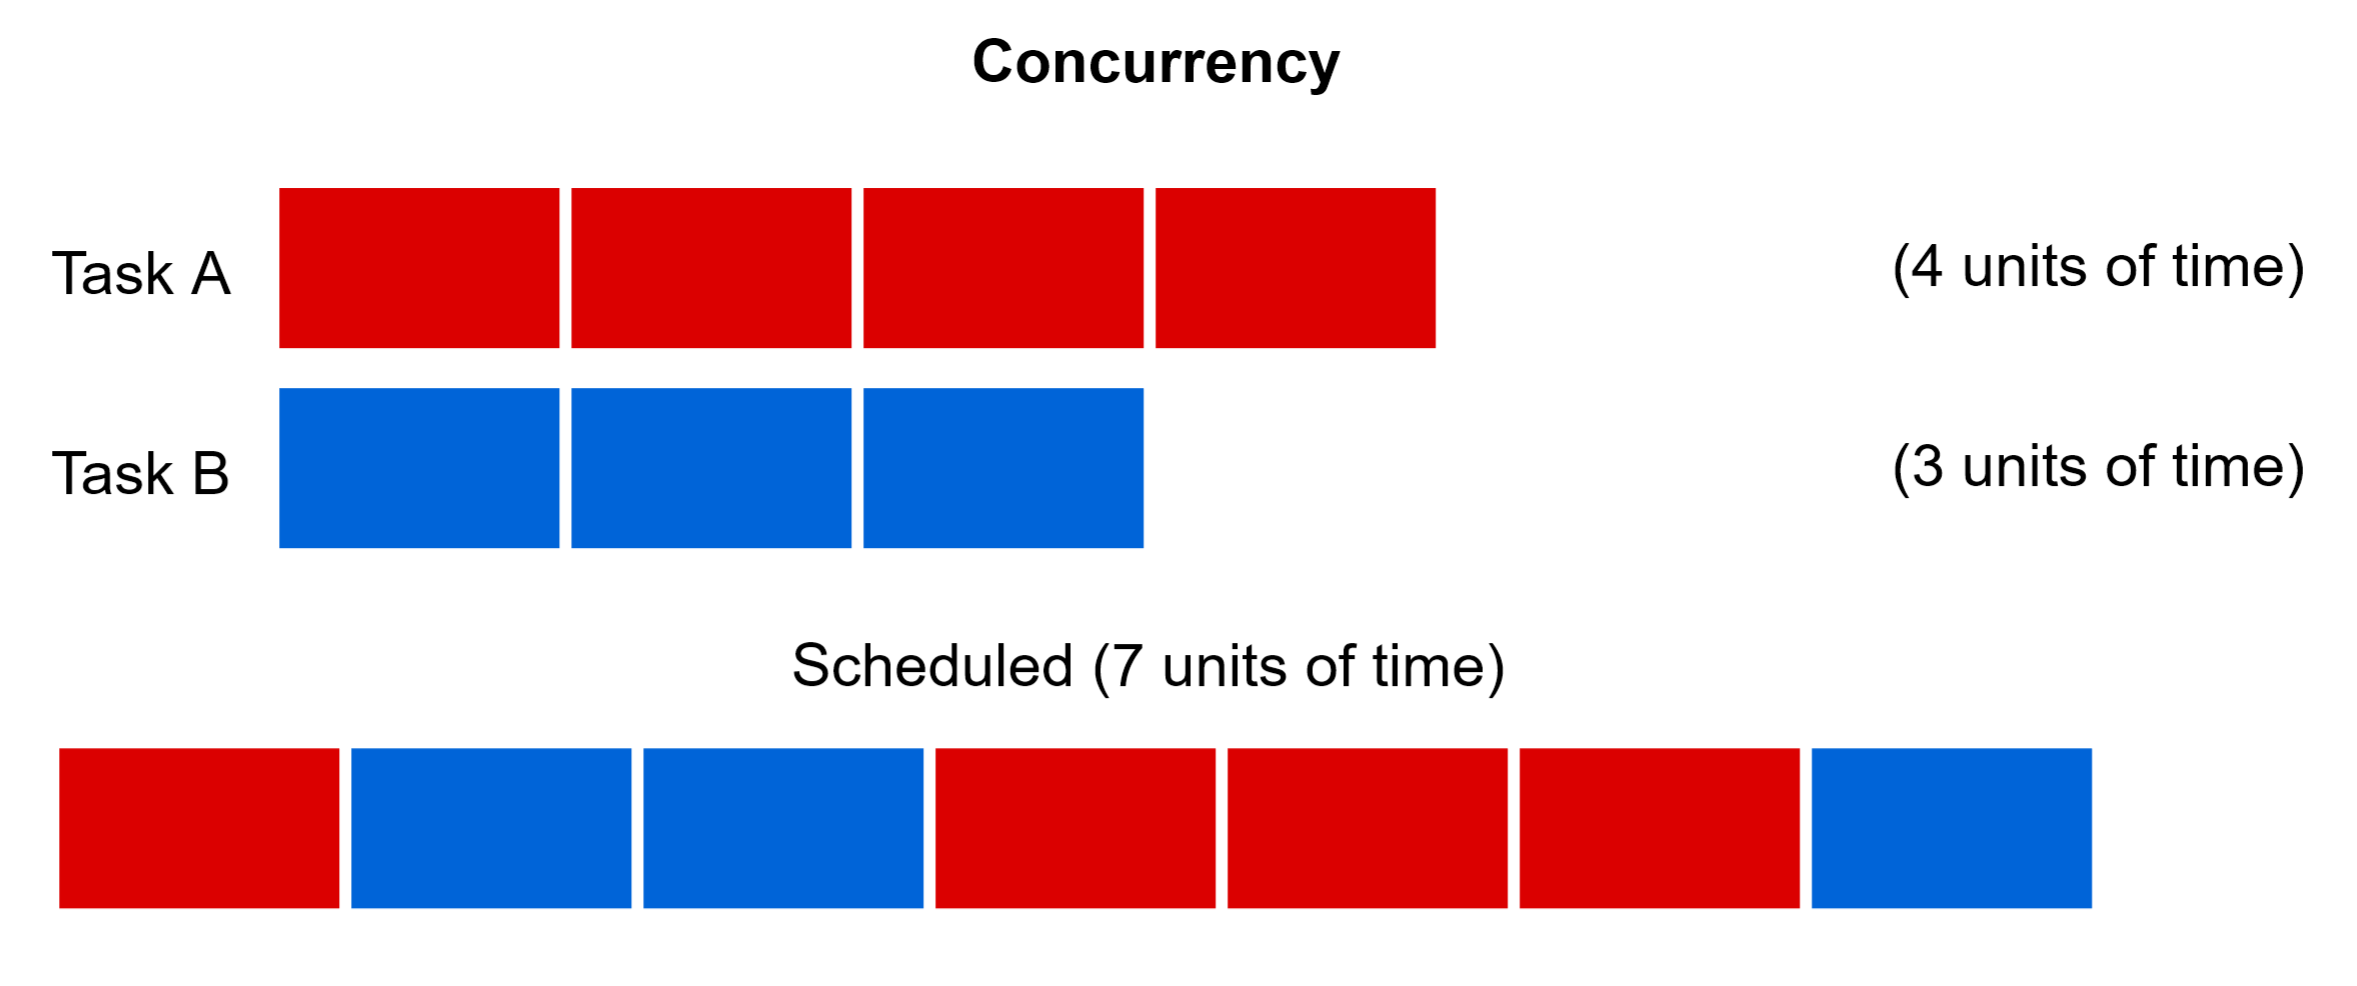
\includegraphics[width=.75\textwidth]{./Sections/high/concurrency.png}
    \caption{Concurrency: Multiple software-threads running on a single hardware-thread.}
\end{figure}

\noindent
In reality, many tasks preform I/O operations, which don't 
concern the CPU:
\begin{figure}[h]
    \centering
    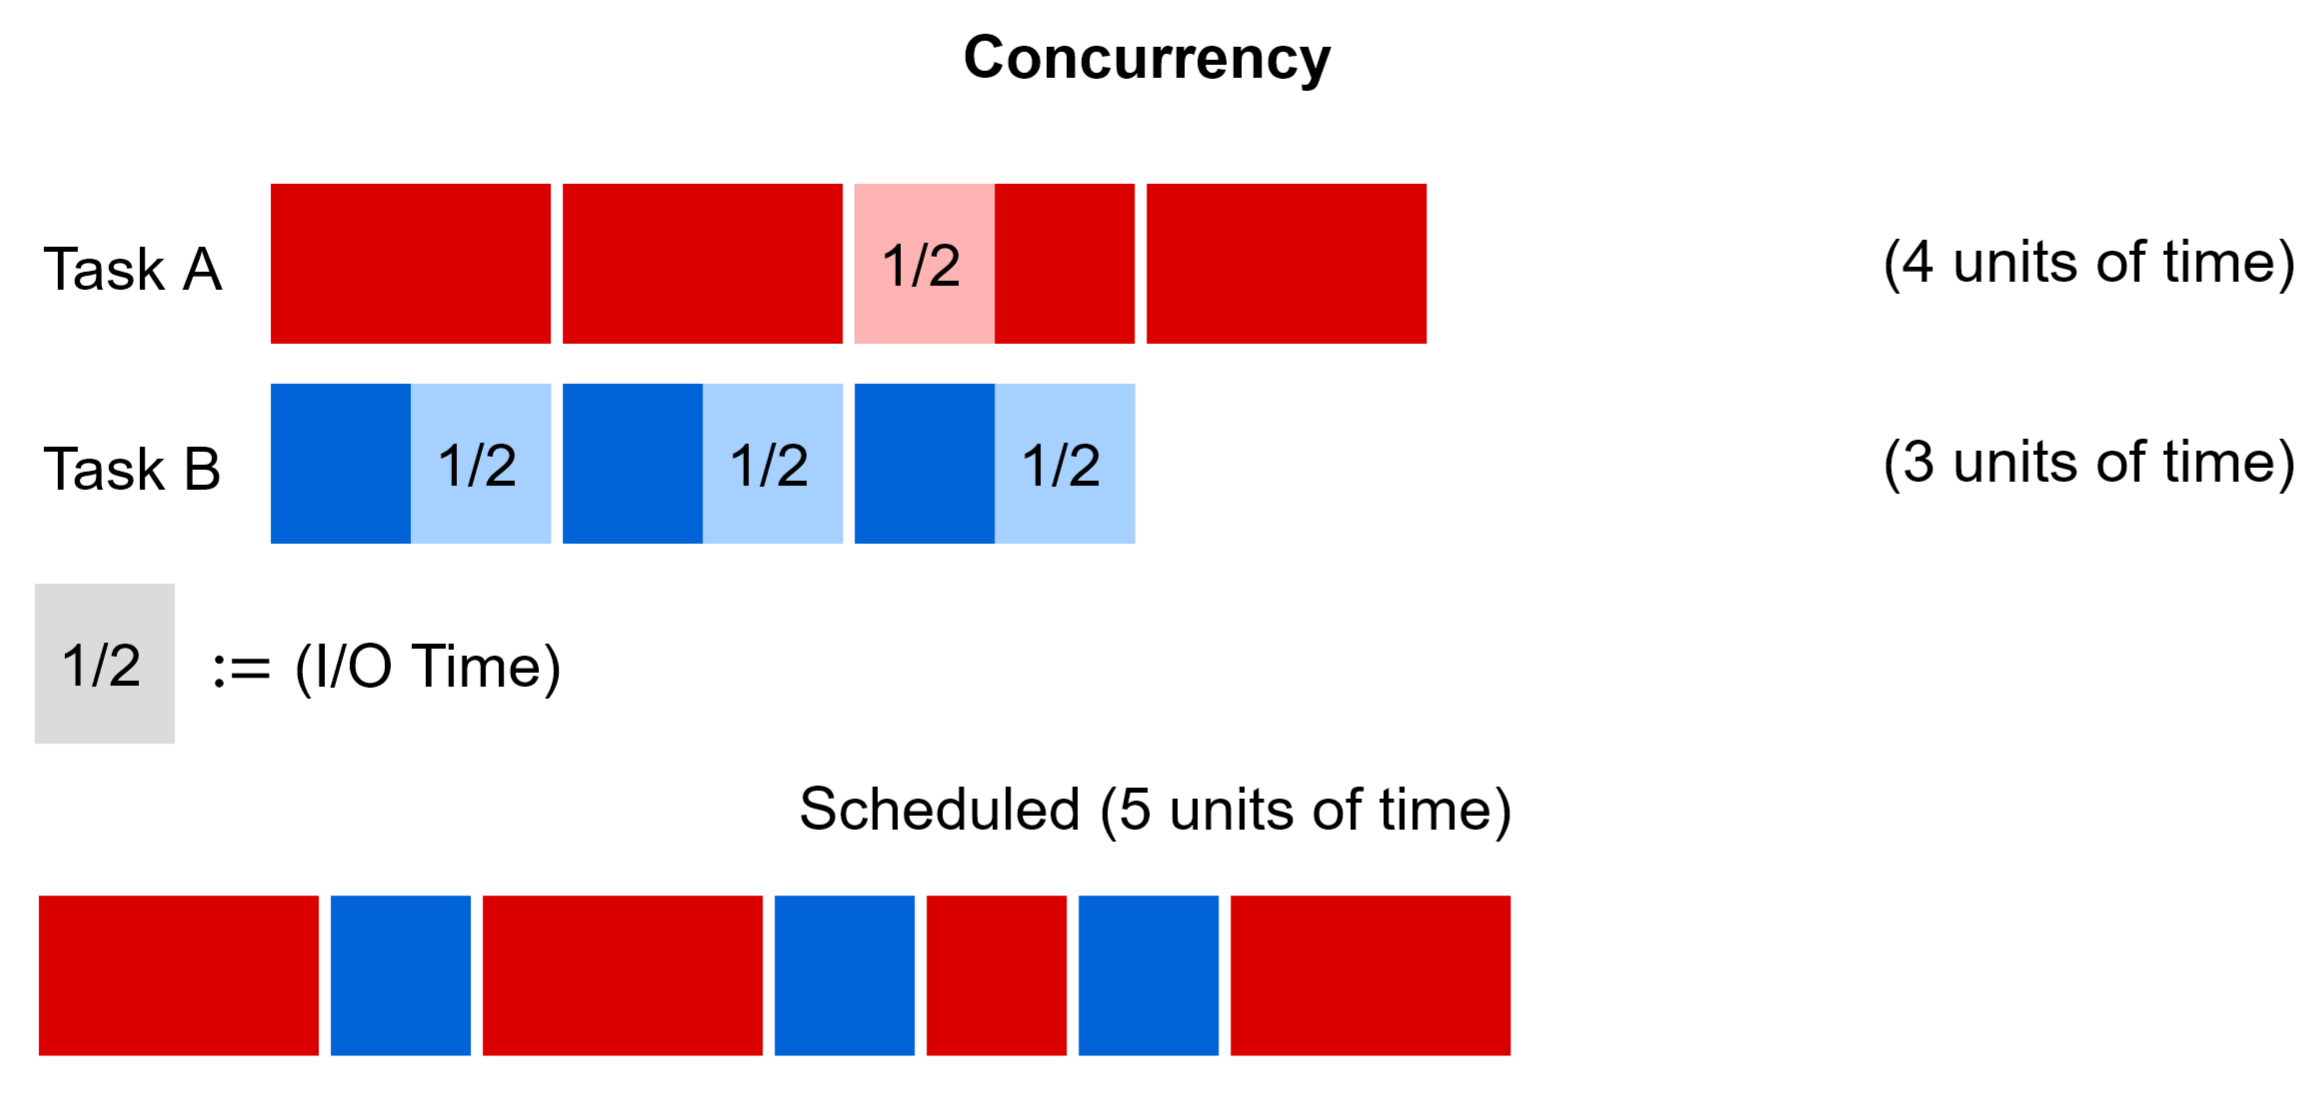
\includegraphics[width=.75\textwidth]{./Sections/high/concurrency_io.png}
    \caption{Concurrency with I/O: Multiple software-threads running on a single hardware-thread.}
\end{figure}

\noindent
Now since the CPU isn't idle on I/O operations, the overall time between tasks is cut significantly.

\newpage

\begin{Def}[Kernel]
    
    The kernel is the central component of the operating system. It manages hardware resources—including the CPU, memory, and I/O devices—and provides core services such as process management, memory management, and device control.
\end{Def}

\begin{figure}[h]
    \centering
    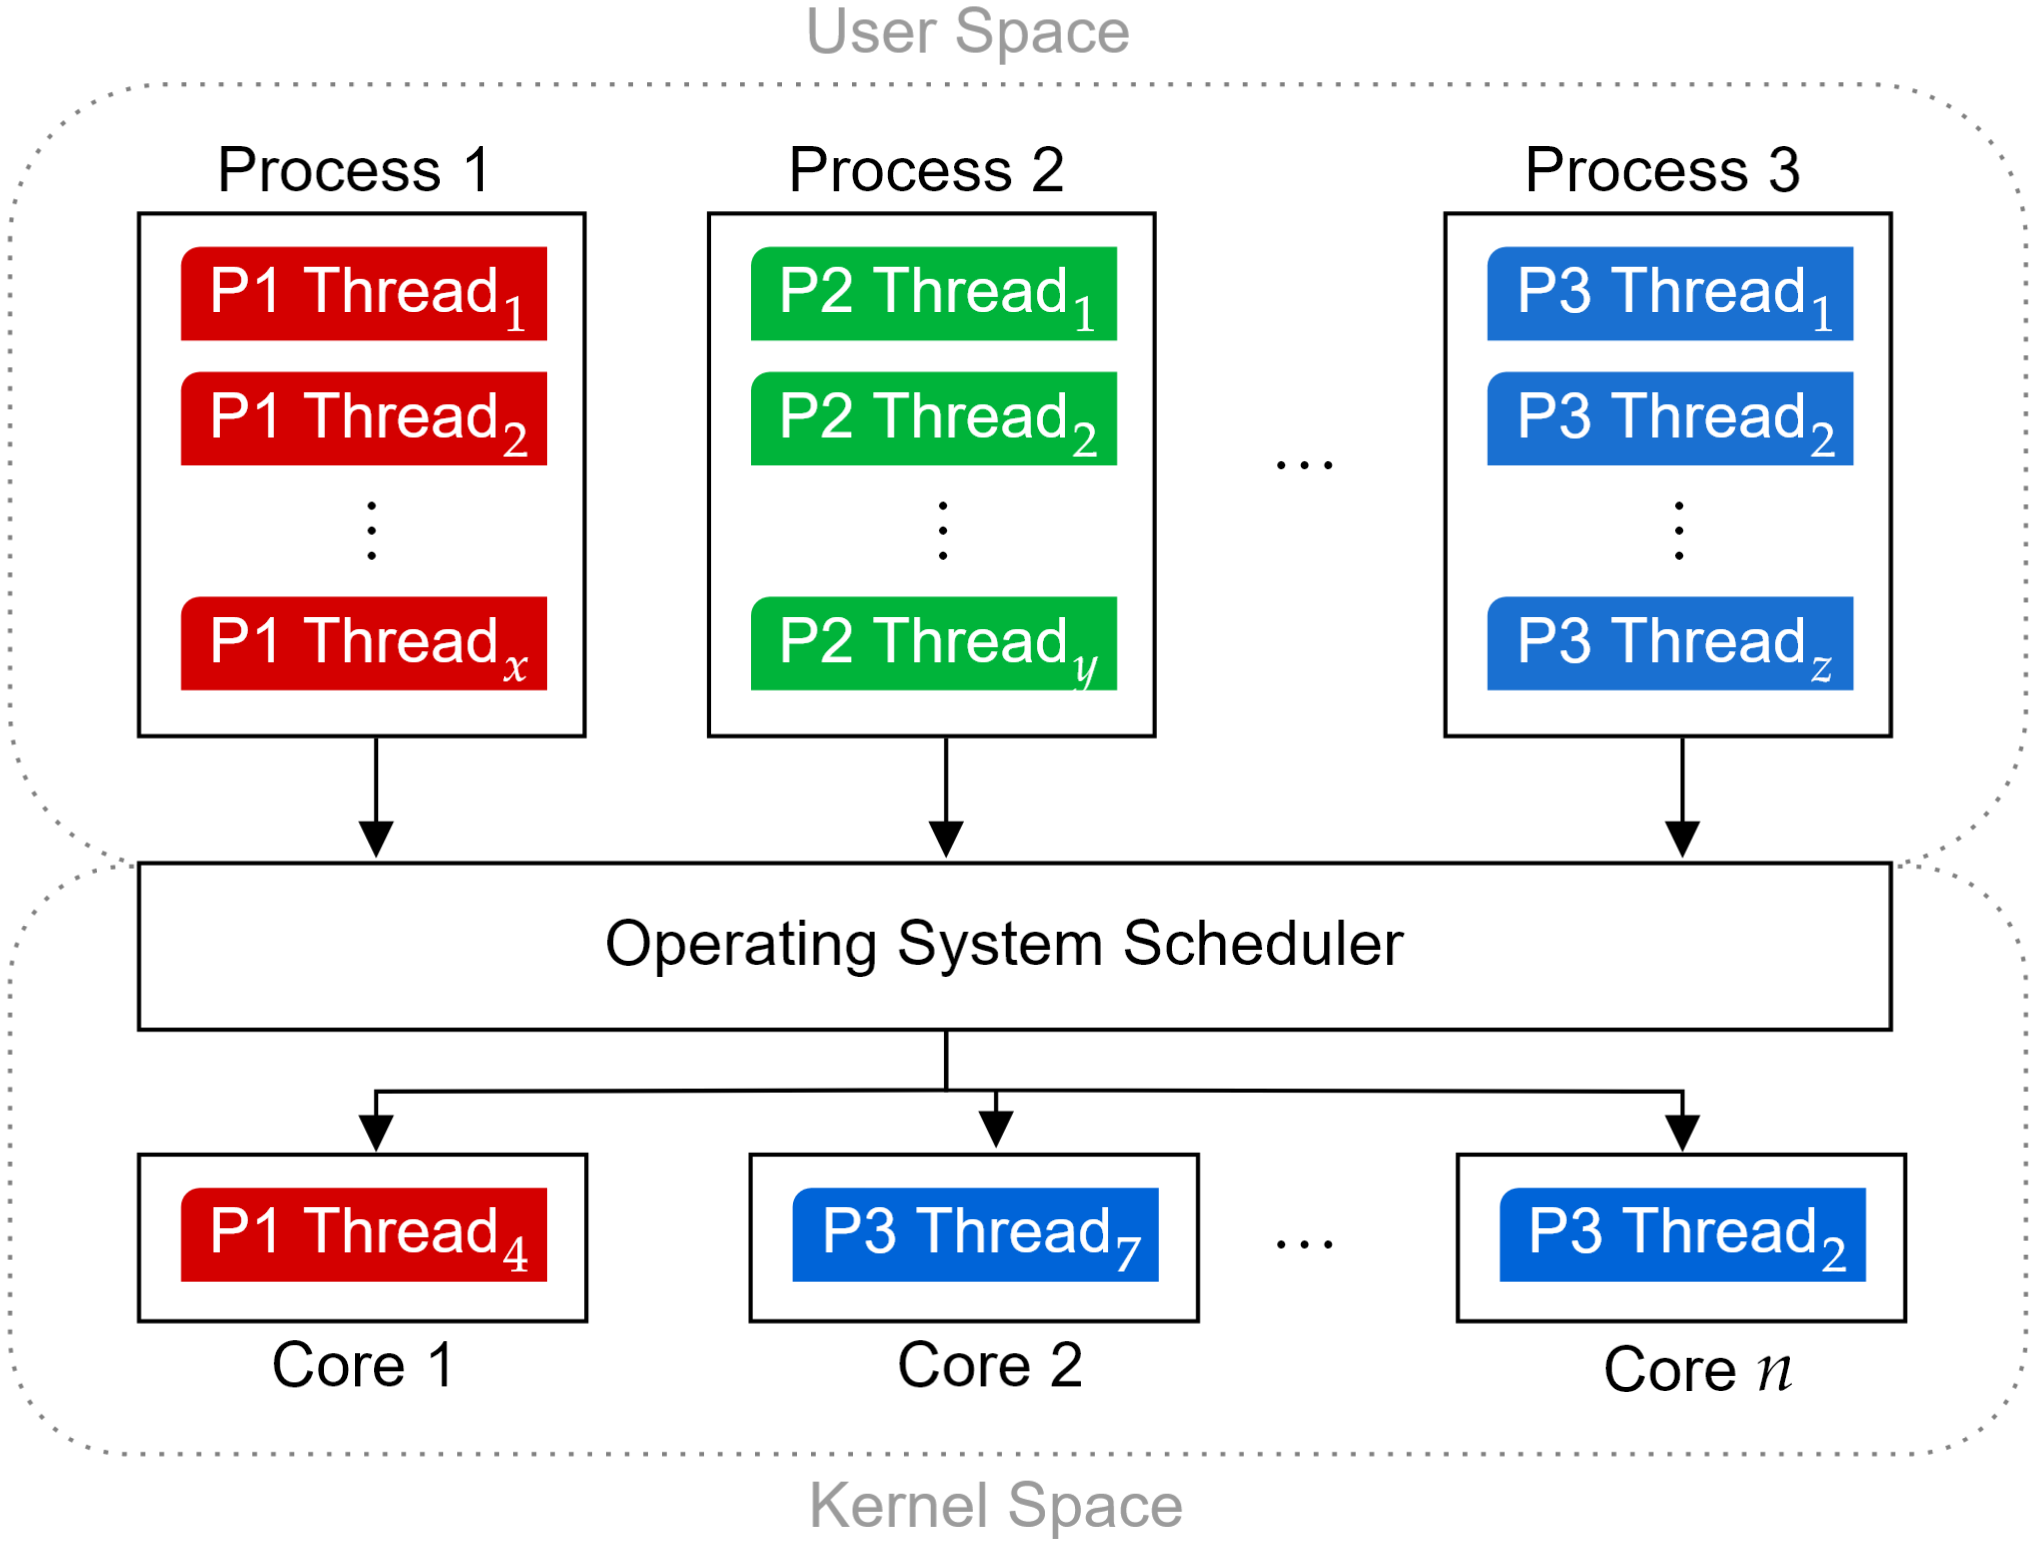
\includegraphics[width=1\textwidth]{./Sections/high/user_kernel.png}
    \caption{Process threads scheduled by the OS kernel and processed by the CPU.}
    \label{fig:kernel}
\end{figure}

\noindent
In summary, what we need to know are these key points:
\begin{itemize}
    \item The CPU executes instructions via processing units called cores/hardware-threads.
    \item The OS schedules software-threads from processes to run on hardware-threads.
    \item A core can only run one software-thread at a time, but can switch between them.
    \item Context switching on a single core is called concurrency, while utilizing multiple cores in unison (multi-threading) is called parallelism.
\end{itemize}


\newpage 

\noindent
\subsection{Motivation for Distributed Systems}

\noindent
Distributed systems cover a vast and diverse range of applications, including:
\begin{itemize}
    \item \textbf{Offloading Computation:} Perhaps a system $A$ offloads a heavy computation to system $B$.
    \item \textbf{Fault Tolerance:} If a critical system $A$ fails, an almost identical system $B$ can take over.
    \item \textbf{Load Balancing:} Say a system $A$ is overwhelmed with requests, it can distribute the load to system $B$, acting as 
    one system, from the requests point of view.
\end{itemize}
In todays market, there are numerous applications of distributed systems, such as:
Cloud Computing, Social Networks, E-commerce, Streaming Services, Search Engines, Renting Computation (AI training), etc.

Let's begin to define the problem space. Say there are 
two individuals Alice and Bob, who wish to communicate:\\
\begin{figure}[h]
    \centering
    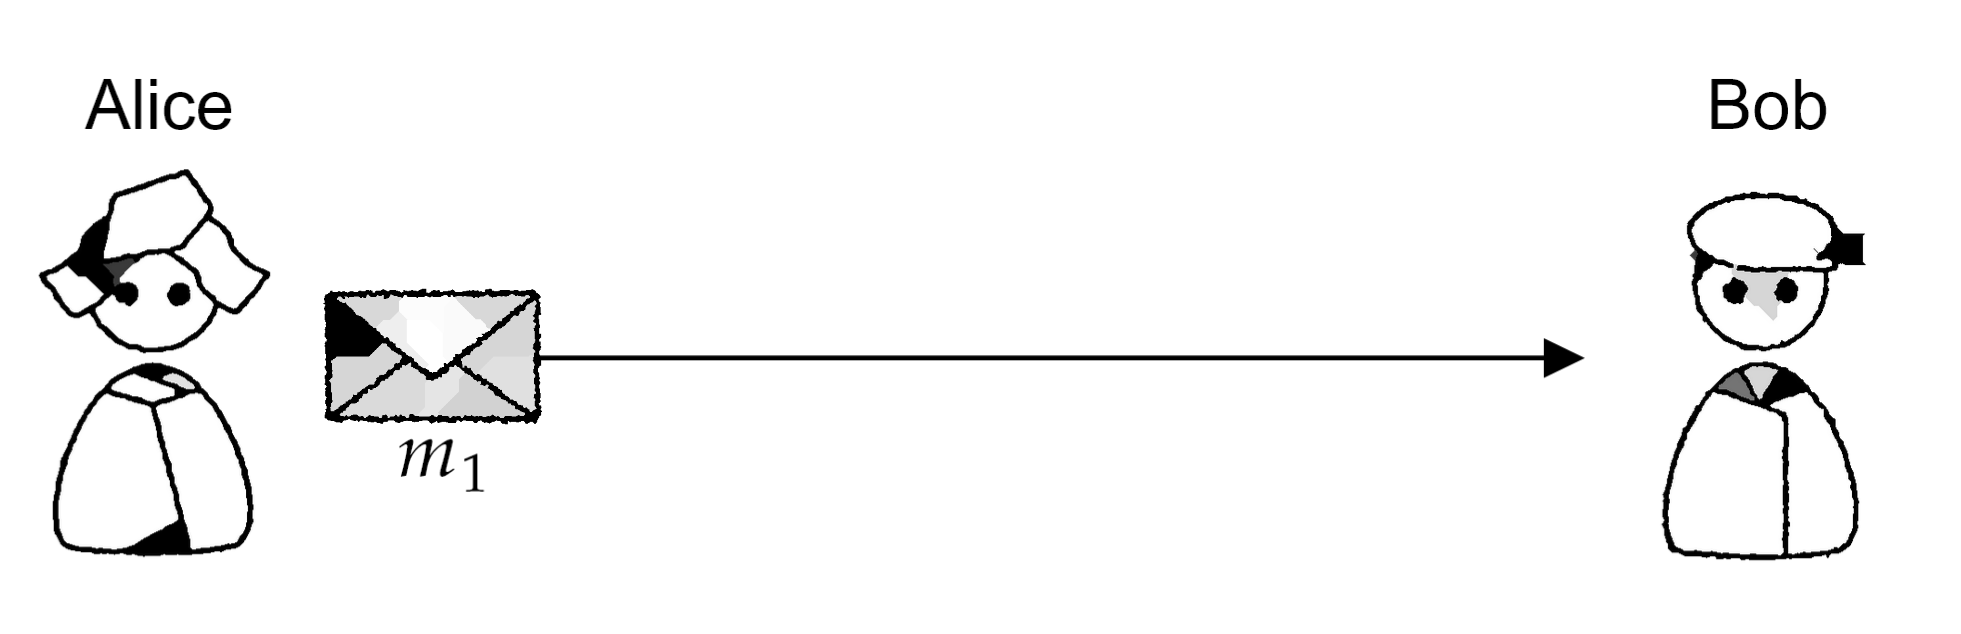
\includegraphics[width=.8\textwidth]{./Sections/high/com.png}
    \caption{Alice sends a letter $m_1$ overseas to Bob.}
\end{figure}

\noindent
How does Alice know that her message $m_1$ was received by Bob? Bob 
would have to send a message back to Alice, acknowledging the receipt of $m_1$.

\begin{figure}[h]
    \centering
    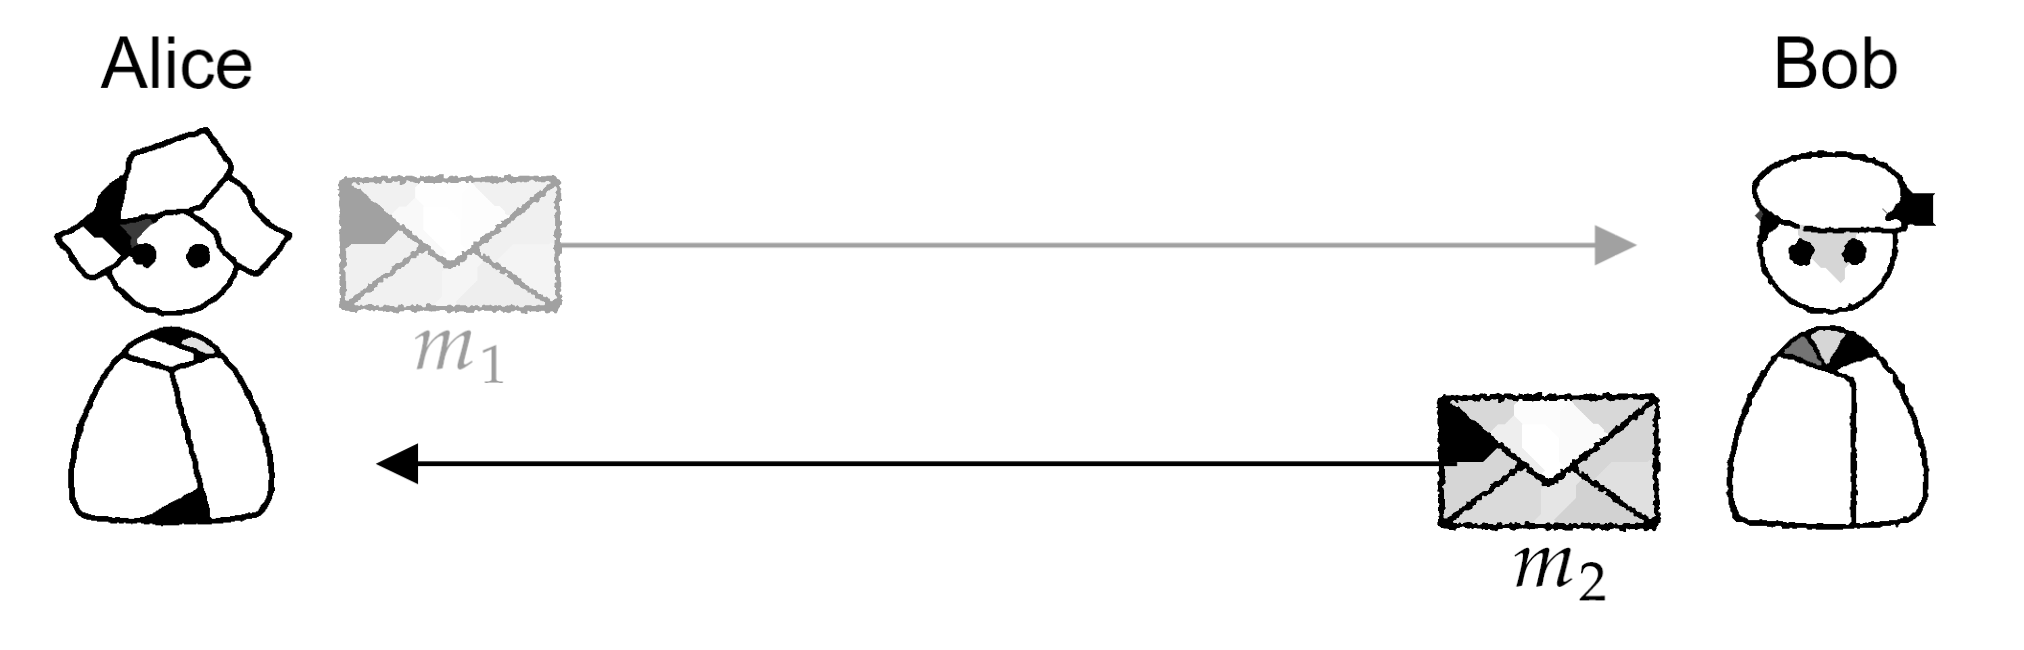
\includegraphics[width=.8\textwidth]{./Sections/high/com_2.png}
    \caption{Bob sends an acknowledgment letter back to Alice.}
\end{figure}
    
\noindent
Though problems can arise, what if Alice's letter gets lost in the mail, what if Bob receives multiple 
letters from Alice, how does Bob know which letter is the most recent? These are the fundamental problems 
of distributed systems.
